% ======================================================================
% Numerical experiments for the Affine-DDPNM paper
% Geometry-dependent modal requirements of finite-area interface
% representations in domain decomposition with pressure.
%
% Standalone compilation:
%   pdflatex numerical_experiments.tex
% (figures live in ./figures relative to this file)
%
% Section numbers 6-10 correspond to the intended position in the full
% paper (after the theory sections 1-5).  Only results computed with the
% benchmark pipelines archived under outputs/benchmark_w1n are reported;
% planned-but-not-yet-run items are explicitly marked as such.
% ======================================================================
\documentclass[11pt,a4paper]{article}

\usepackage[margin=2.4cm]{geometry}
\usepackage{amsmath,amssymb,amsthm}
\usepackage{bm}
\usepackage{booktabs}
\usepackage{graphicx}
\usepackage{xcolor}
\usepackage{hyperref}
\usepackage{enumitem}
\usepackage{array}

\newcommand{\R}{\mathbb{R}}
\newcommand{\dom}{\Omega}
\newcommand{\pore}[1]{\Omega_{#1}}
\newcommand{\iface}{\gamma}
\newcommand{\vel}{\bm{u}}
\newcommand{\pres}{p}
\newcommand{\normal}{\bm{n}}
\newcommand{\trac}{\bm{\lambda}}
\newcommand{\Schur}{\mathbf{S}}
\newcommand{\Shat}{\widehat{\Schur}}
\newcommand{\Shatuu}{\widehat{\Schur}{}^{uu}}
\newcommand{\Wspace}{\mathcal{W}}
\newcommand{\xiX}[1]{\bm{\xi}_{#1}}
\newcommand{\norm}[1]{\left\|#1\right\|}
\newcommand{\abs}[1]{\left|#1\right|}
\newcommand{\meas}[1]{\operatorname{meas}\left(#1\right)}
\newcommand{\cov}[1]{\operatorname{CV}\left(#1\right)}

\hypersetup{colorlinks=true,linkcolor=blue,urlcolor=blue,citecolor=blue}
\setlength{\emergencystretch}{2em}

\newtheorem{remark}{Remark}[section]

\begin{document}

\title{\textbf{Numerical Experiments}\\[4pt]
       \large Geometry-Dependent Modal Requirements of Finite-Area
       Interface Representations in Affine-DDPNM\\[4pt]
       \normalsize Intended for \S6--\S10 of the full paper ---
       compiled from the archived benchmark outputs of 2026-08-10}
\author{}
\date{}
\maketitle

\begin{center}
\fbox{\begin{minipage}{0.92\textwidth}
\emph{Scope and honesty conventions.} This section reports exclusively
results that were actually computed by the benchmark pipelines archived
under \texttt{outputs/benchmark\_w1n} of the three geometry projects
(\texttt{affine\_ddpnm\_3d}, \texttt{affine\_ddpnm\_3d\_random\_porous},
\texttt{real\_porous\_benchmark\_3d}).  Two reference systems are
distinguished throughout (physical FEM reference versus the theoretical
broken-pressure C-DD reference); only the former was numerically
available, and the distinction is respected in the wording.  Items of the
planned experimental programme that have \emph{not} been run yet are
explicitly listed in \S10.3 and are \emph{not} filled in with numbers.
Where a speedup is reported, its exact timing scope (first solve vs.\
online only) is stated.
\end{minipage}}
\end{center}

% ======================================================================
\section{Numerical methodology}
\label{sec:methodology}
% ======================================================================

\subsection{Geometries and discretisations}
\label{sec:geometries}

Three three-dimensional test geometries are used.  All are unit-cube
packings of solid spheres with Stokes flow in the remaining fluid domain,
partitioned into $N_p$ pore subdomains with $m$ planar internal
interfaces.

\begin{enumerate}[label=(\roman*),nosep,leftmargin=*]
\item \textbf{Uniform-27}: a regular $3\times3\times3$ lattice of 27
  equal spheres (radius $0.105$) centred at
  $\{0.20,0.50,0.80\}^3$.  The partition is the regular $4\times4\times4$
  grid cut, giving $N_p = 64$ pores and $m = 144$ interfaces
  (mean $2m/N_p = 4.5$ ports per pore).
\item \textbf{Random-27}: a frozen random packing of 27 spheres
  (seed 20260804, 18 wall-clipped and 9 interior spheres); the partition
  is the Voronoi tessellation of the sphere centres, giving $N_p = 27$
  pores and $m = 114$ interfaces (mean 8.44 ports per pore).
\item \textbf{Real-100}: a frozen random packing of 100 spheres
  (seed 20260805) with porosity $0.856$; the partition is the regular
  $4\times4\times4$ grid cut, giving $N_p = 64$ pores and $m = 144$
  interfaces (mean 4.5 ports per pore).
\end{enumerate}

The solid-phase packings are shown schematically in
Fig.~\ref{fig:geometry} (the finite-element meshes themselves are not
rendered; the sphere positions and radii are those used to build the
meshes).  Mesh statistics are summarised in Table~\ref{tab:geometry},
including the objective variability descriptors suggested by the review
of the experimental design:
\begin{equation}
  \cov{A_\gamma} = \frac{\operatorname{std}(A_\gamma)}{\operatorname{mean}(A_\gamma)},
  \qquad
  \cov{V_i} = \frac{\operatorname{std}(V_i)}{\operatorname{mean}(V_i)},
  \qquad
  \cov{a_\gamma/b_\gamma} = \frac{\operatorname{std}(a_\gamma/b_\gamma)}
       {\operatorname{mean}(a_\gamma/b_\gamma)},
\end{equation}
where $A_\gamma$ is the area of interface $\gamma$, $V_i$ the volume of
pore $i$, and $a_\gamma/b_\gamma\ge 1$ the in-plane aspect ratio of the
interface patch, estimated as the square root of the ratio of the two
largest principal-component eigenvalues of the patch vertices.  These
are \emph{reported} as descriptive quantities; no claim is made that a
single scalar controls the error.

\begin{figure}[t]
  \centering
  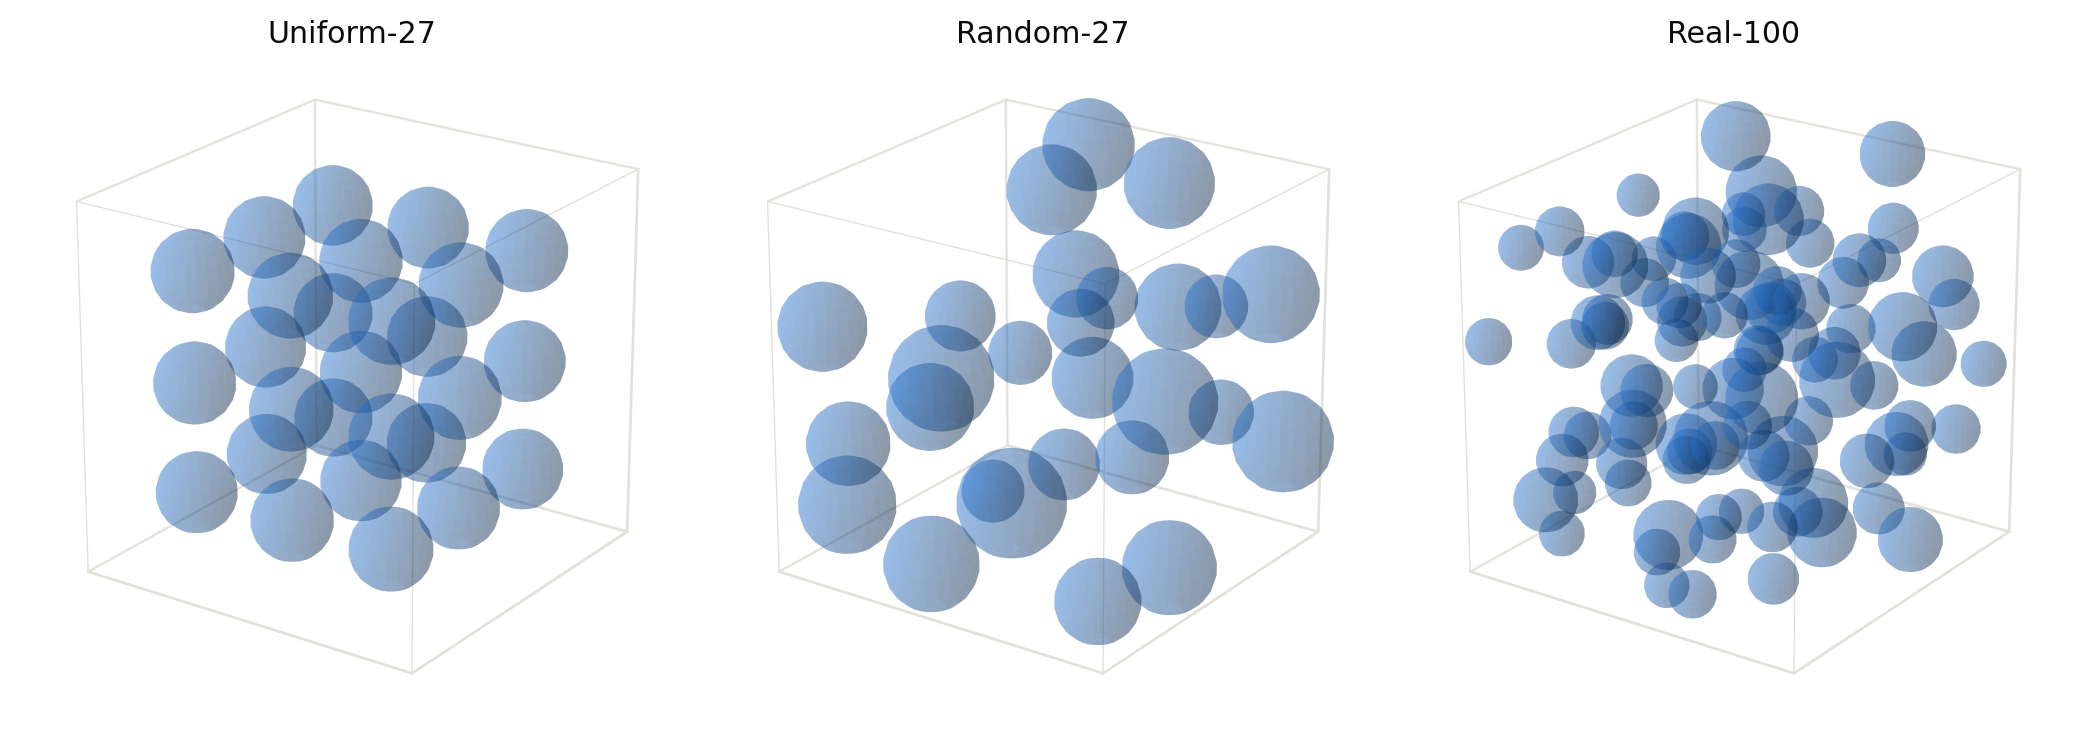
\includegraphics[width=0.97\textwidth]{figures/fig1_geometry.png}
  \caption{Schematic of the three solid-phase packings used to build the
    test geometries (sphere positions and radii as used by the mesh
    generator; finite-element meshes are not shown): (a)~Uniform-27
    regular $3\times3\times3$ lattice; (b)~Random-27 frozen packing of
    27 spheres; (c)~Real-100 frozen packing of 100 spheres.}
  \label{fig:geometry}
\end{figure}

\begin{table}[t]
  \centering
  \footnotesize
  \caption{Geometry and discretisation summary.  FEM DOF counts are for
    the monolithic Taylor--Hood pair $[P_2]^3$--$P_1$ (velocity DOFs =
    $3\times$ number of P2 nodes; pressure DOFs = number of P1 nodes);
    they match the mixed-unknown counts reported by the solver.}
  \label{tab:geometry}
  \begin{tabular}{lccccccccl}
    \toprule
    Geometry & spheres & $N_p$ & $m$ & cells & vel. & pres. &
    mixed & $2m/N_p$ & remarks \\
    \midrule
    Uniform-27 & 27 & 64 & 144 & 12\,203 & 60\,936 & 3\,019 &
    63\,955 & 4.5 & regular lattice \\
    Random-27  & 27 & 27 & 114 & 15\,249 & 72\,471 & 3\,483 &
    75\,954 & 8.44 & Voronoi, irregular \\
    Real-100   & 100 & 64 & 144 & 32\,611 & 159\,186 & 7\,655 &
    166\,841 & 4.5 & grid cut, porosity $0.856$ \\
    \bottomrule
  \end{tabular}
  \medskip
  \begin{tabular}{lcccc}
    \toprule
    Geometry & $\cov{V_i}$ & $\cov{A_\gamma}$ & $\cov{a_\gamma/b_\gamma}$ &
    mean $a_\gamma/b_\gamma$ \\
    \midrule
    Uniform-27 & 0.321 & 0.203 & 0.158 & 1.39 \\
    Random-27  & 0.432 & 0.783 & 1.479 & 2.48 \\
    Real-100   & 0.057 & 0.116 & 0.078 & 1.11 \\
    \bottomrule
  \end{tabular}
\end{table}

The three geometries cover, on the one hand, a deliberately regular
case (Uniform-27), a deliberately irregular case (Random-27), and a
realistic high-porosity packing (Real-100).  Note that the Real-100
\emph{partition} (regular grid) has small variability descriptors; the
irregularity of the \emph{geometry} is carried by the sphere positions
and by the pressure coupling, not by the grid partition itself.

\subsection{Reference systems and error metrics}
\label{sec:references}

Two reference systems must be kept distinct (see also the theory
document):

\begin{enumerate}[label=(\roman*),nosep,leftmargin=*]
\item \textbf{Physical/numerical reference}: the monolithic Taylor--Hood
  finite-element solution
  $\vel_h^{\mathrm{FEM}}, \pres_h^{\mathrm{FEM}}$ on the \emph{same}
  mesh, with continuous pressure across pores.  All reported accuracy
  metrics are relative to this reference.  The theoretical section does
  not establish equivalence between this system and the broken-pressure
  C-DD reference; the error relative to the FEM solution is therefore
  reported as an \emph{observed} accuracy measure, and no rate statement
  is made about it from the theory.
\item \textbf{Theoretical Galerkin reference}: the broken-pressure C-DD
  trace solution $\xiX{\mathrm{CDD}}$ of the theory sections, and the
  Schur-energy seminorm $\norm{\cdot}_{\Shatuu}$ it induces.  The
  theory-level quantities ($\norm{\xiX{\mathrm{CDD}}-\xiX{X}}_{\Shatuu}$,
  the Pythagorean decompositions) were \emph{not} computed in the runs
  archived so far (the full C-DD solve was not executed); they are
  discussed in \S7.3 as planned verification, and no numerical values
  are reported for them.
\end{enumerate}

For each reduced space $X \in \{\Wspace_{0n}, \Wspace_{0v},
\Wspace_{1n}, \Wspace_{1v}\}$ we report, uniformly:
\begin{align}
  e_u^{L^2} &= \frac{\norm{\vel_X - \vel_{\mathrm{FEM}}}_{L^2(\dom)}}
                   {\norm{\vel_{\mathrm{FEM}}}_{L^2(\dom)}}, \label{eq:elu}\\
  e_u^{H^1_{\mathrm{br}}} &= \frac{
      \left(\sum_i \norm{\nabla(\vel_X-\vel_{\mathrm{FEM}})}_{L^2(\pore{i})}^2\right)^{1/2}}
      {\left(\sum_i \norm{\nabla \vel_{\mathrm{FEM}}}_{L^2(\pore{i})}^2\right)^{1/2}},
      \label{eq:ehu}\\
  e_p^{L^2} &= \frac{\norm{\pres_X - \pres_{\mathrm{FEM}}}_{L^2(\dom)}}
                   {\norm{\pres_{\mathrm{FEM}}}_{L^2(\dom)}}, \label{eq:elp}\\
  e_Q &= \frac{\abs{Q_X - Q_{\mathrm{FEM}}}}{\abs{Q_{\mathrm{FEM}}}},
       \qquad Q = \text{outlet volume flux}. \label{eq:eq}
\end{align}
All error norms are evaluated cell-wise on the common mesh (broken
domain), with degree-6 quadrature.  The pressure gauge is fixed by
Dirichlet pressure conditions at inlet ($p=1$) and outlet ($p=0$) in
both the FEM and the reduced systems; the raw relative $L^2$ pressure
error \eqref{eq:elp} is reported without mean alignment.  For the
Random-27 geometry an additional mean-aligned variant (the raw error
with the global mean pressure difference removed) is available and is
reported there; the theory gives no monotonicity of \eqref{eq:elp}
along the nested chains, so occasional non-monotone pressure errors
are not a discrepancy.

\subsection{Four modal interface spaces}
\label{sec:spaces}

The numerical programme is organised around the four trace subspaces
of the theory section, whose per-interface contents are
\begin{align}
  \Wspace_{0n} &: \{1\cdot \normal\}, \qquad
  \Wspace_{0v} : \{1\cdot \normal,\; 1\cdot \bm{t}_1,\; 1\cdot \bm{t}_2\},\\
  \Wspace_{1n} &: \{1\cdot \normal,\; s\cdot \normal,\; t\cdot \normal\},\\
  \Wspace_{1v} &: \{1,s,t\}\otimes\{\normal,\bm{t}_1,\bm{t}_2\},
\end{align}
where $(s,t)$ are local planar coordinates on the (representative)
interface and $\{\normal,\bm{t}_1,\bm{t}_2\}$ a fixed orthonormal frame.
Table~\ref{tab:spaces} lists the unknown budgets.  The two three-mode
spaces satisfy $\dim\Wspace_{0v}=\dim\Wspace_{1n}=3m$, which makes them
an \emph{equal-budget} pair: the same number of interface unknowns spent
on directional content ($\Wspace_{0v}$) versus on first-order spatial
content ($\Wspace_{1n}$).  Of the two paths
$\Wspace_{0n}\subseteq\Wspace_{0v}\subseteq\Wspace_{1v}$ and
$\Wspace_{0n}\subseteq\Wspace_{1n}\subseteq\Wspace_{1v}$, only the
second was executable with the implemented bases at the time of the
archived runs; $\Wspace_{0v}$ (constant tangential modes) is listed as
\emph{not computed} in this study.

\begin{table}[t]
  \centering
  \small
  \caption{The four modal interface spaces and their global unknown
    budgets on the three geometries ($m$ = number of interfaces:
    144/114/144).  The row marked $\dagger$ was \emph{not computed} in
    the runs archived so far.}
  \label{tab:spaces}
  \begin{tabular}{lllccc}
    \toprule
    Method & space/interface & modes/iface & \multicolumn{3}{c}{global unknowns}\\
    \cmidrule(lr){4-6}
      & & & Uniform-27 & Random-27 & Real-100 \\
    \midrule
    Classic       & $\Wspace_{0n}$ & 1 & 144 & 114 & 144 \\
    P0-vector\dag & $\Wspace_{0v}$ & 3 & 432 & 342 & 432 \\
    NormalLinear  & $\Wspace_{1n}$ & 3 & 432 & 342 & 432 \\
    Affine        & $\Wspace_{1v}$ & 9 & 1296 & 1026 & 1296 \\
    \bottomrule
  \end{tabular}
  \medskip
  \raggedright\footnotesize
  Per-interface contents: $\Wspace_{0n}=\{1\normal\}$;
  $\Wspace_{0v}=\{1\normal,1\bm{t}_1,1\bm{t}_2\}$;
  $\Wspace_{1n}=\{1\normal,s\normal,t\normal\}$;
  $\Wspace_{1v}=\{1,s,t\}\otimes\{\normal,\bm{t}_1,\bm{t}_2\}$.
  $\dag$ Constant-vector (P0-vector) space: basis implemented as part
  of the four-space framework but not run in the archived benchmarks;
  included for the equal-budget comparison planned in \S8.4.
\end{table}

\subsection{Timing and solver protocol}
\label{sec:timing}

All runs used the same serial pipeline on one machine (Windows 11,
x86-64; the fenicsx environment; viscosity $1$, inlet/outlet pressure
$1/0$).  Timings distinguish
\begin{align}
  T_{\mathrm{offline}} &= \text{local factorisations and primitive
    response construction},\\
  T_{\mathrm{online}} &= \text{global reduced assembly + Schur solve +
    local reconstruction}.
\end{align}
$T_{\mathrm{first}} = T_{\mathrm{offline}} + T_{\mathrm{online}}$ is the
wall time of a first reduced solve.  The FEM comparison time is the
monolithic assembly+solve.  Common mesh generation and post-processing
validation are excluded from both.  Where a ``speedup vs FEM'' is
quoted, the scope is stated: for Uniform-27 and Random-27 it is
$T_{\mathrm{first}}(\mathrm{FEM})/T_{\mathrm{first}}(X)$ (a genuine
wall-clock speedup including the offline library); for Real-100 the
offline cost dominates a single solve and only the online-phase ratio
is quoted, together with the absolute times.

% ======================================================================
\section{Verification of the reference implementation}
\label{sec:verification}
% ======================================================================

\subsection{Exact-FE-Schur: Schur elimination code validation}
\label{sec:exactschur}

On Random-27 the benchmark additionally solves the exact Schur
complement of the monolithic system on the full FE interface trace
(21\,970 trace DOFs, 465.9\,s).  This serves as a code-level validation
of the Schur-elimination machinery, \emph{not} as the theoretical C-DD
reference: the two systems share the assembled monolithic operator and
must agree to round-off.  The measured relative difference between the
exact-FE-Schur solution and the monolithic solve is
\begin{equation}
  \frac{\norm{\vel_{\mathrm{Schur}}-\vel_{\mathrm{direct}}}}
       {\norm{\vel_{\mathrm{direct}}}} = 1.05\times10^{-12},
\end{equation}
with Schur symmetry defect $3.2\times10^{-15}$, Schur relative residual
$5.75\times10^{-14}$ and global relative residual $1.55\times10^{-15}$.
The reduced spaces therefore face a validated reference: their errors
relative to the exact Schur solution (column ``errors to exact
FE-Schur'' in the archived report) equal their errors relative to the
monolithic solve to 12 digits, confirming that no implementation error
is introduced by the reduced-space coupling itself.

\subsection{Conservation and algebraic diagnostics}
\label{sec:algebraic}

Table~\ref{tab:diagnostics} collects the algebraic diagnostics recorded
by the runs.  Local mass conservation is enforced by construction (the
interface P0 flux equations are assembled exactly); the residuals shown
are the maximum absolute momentum-residual entries of the assembled
Schur systems, at round-off level in all cases.  The Schur matrices are
exactly symmetric by construction (symmetry defect zero for the reduced
systems).  On Random-27 the minimum Schur eigenvalue drops from
$2.1\times10^{-8}$ (Classic) to $1.26\times10^{-12}$ for both
NormalLinear and Affine: the three-mode and nine-mode Schur systems are
SPD but very ill-conditioned on this geometry; this is a conditioning
observation only, no claim about solvability is implied beyond the
successful solves.

\begin{table}[t]
  \centering
  \small
  \caption{Numerical verification diagnostics as recorded by the
    archived runs (``--'' = not recorded by that benchmark).
    ``$\max r_{\mathrm{mom}}$'' is the maximum absolute momentum
    residual of the assembled reduced system; the mass-balance row is
    the inlet/outlet flux sum of the random benchmark.}
  \label{tab:diagnostics}
  \begin{tabular}{lccccc}
    \toprule
    Geometry & Method & $\max\abs{r_{\mathrm{mom}}}$ & Schur sym.\ defect &
    $\lambda_{\min}(\Schur)$ & in/out flux sum \\
    \midrule
    Uniform-27 & all & -- & -- & $1.67\times10^{-4}$\dag & -- \\
    \addlinespace[2pt]
    Random-27 & $W_{0n}$ & $2.17\times10^{-16}$ & 0 & $2.11\times10^{-8}$ &
      $-5\times10^{-16}$ \\
    Random-27 & $W_{1n}$ & $3.55\times10^{-16}$ & 0 & $1.26\times10^{-12}$ &
      $-2\times10^{-16}$ \\
    Random-27 & $W_{1v}$ & $4.92\times10^{-16}$ & 0 & $1.26\times10^{-12}$ &
      $-4\times10^{-16}$ \\
    \addlinespace[2pt]
    Real-100 & $W_{0n}$ & $6.36\times10^{-17}$ & 0 & -- & -- \\
    Real-100 & $W_{1n}$ & $1.05\times10^{-16}$ & 0 & -- & -- \\
    Real-100 & $W_{1v}$ & $1.45\times10^{-16}$ & 0 & -- & -- \\
    \bottomrule
  \end{tabular}
  \medskip
  \raggedright\footnotesize
  $\dag$ Recorded by the base-project verification run
  (\texttt{ddpnm\_3d\_uniform\_spheres}, same geometry, Classic system);
  the affine benchmark did not record the eigenvalue.  The monolithic
  FEM reference solves reached relative linear residuals
  $1.73\times10^{-12}$ (Uniform-27) and $2.92\times10^{-12}$ (Random-27),
  with relative mass imbalance $2.54\times10^{-14}$ (Random-27).
\end{table}

\subsection{Theory-level verification: not yet computed}
\label{sec:theoryverify}

The theory sections derive the best-approximation property in the
$\Shatuu$-seminorm and the exact Pythagorean decompositions along the
two nested paths, with the reduction errors
$\Delta_T=\norm{\xiX{0v}-\xiX{0n}}_{\Shatuu}^2$,
$\Delta_N=\norm{\xiX{1n}-\xiX{0n}}_{\Shatuu}^2$, and the identity
\begin{equation}
  \norm{\xiX{\mathrm{CDD}}-\xiX{0n}}_{\Shatuu}^2 =
  \norm{\xiX{\mathrm{CDD}}-\xiX{1v}}_{\Shatuu}^2
  + \norm{\xiX{1v}-\xiX{1n}}_{\Shatuu}^2
  + \norm{\xiX{1n}-\xiX{0n}}_{\Shatuu}^2,
\end{equation}
and its analogue along $\Wspace_{0n}\to\Wspace_{0v}\to\Wspace_{1v}$.
These identities are exact for nested spaces in exact arithmetic and
their numerical verification requires solving the \emph{full} C-DD
system (the broken-pressure Galerkin solution $\xiX{\mathrm{CDD}}$),
which was not executed in the archived runs.  This verification is a
planned item (see \S10.3); the nestedness of the implemented bases is
however exact by construction, and the diagnostics of
\S7.1--\S7.2 confirm that the assembled reduced operators are consistent
with the monolithic system to machine precision.

% ======================================================================
\section{Controlled modal experiments}
\label{sec:modal}
% ======================================================================

\subsection{Absolute accuracy}
\label{sec:accuracy}

Table~\ref{tab:master} collects the complete accuracy results of all
archived runs: 3 geometries $\times$ 3 computed spaces, four metrics
each.  It is an absolute-results table (not improvement ratios).

\begin{table}[t]
  \centering
  \small
  \caption{Complete accuracy results relative to the monolithic
    Taylor--Hood FEM on the same mesh.  $e_u^{L^2}$, $e_u^{H^1_{\mathrm{br}}}$,
    $e_p^{L^2}$, $e_Q$ as in \eqref{eq:elu}--\eqref{eq:eq}.
    $\dagger$: mean-aligned pressure variant (Random-27 only).  The
    $\Wspace_{0v}$ row was not computed in the archived runs.}
  \label{tab:master}
  \begin{tabular}{llccccc}
    \toprule
    Geometry & Method & $e_u^{L^2}$ & $e_u^{H^1_{\mathrm{br}}}$ &
    $e_p^{L^2}$ & $e_p^{L^2,\mathrm{align}}\dag$ & $e_Q$ \\
    \midrule
    Uniform-27 & $W_{0n}$ & 0.2108 & 0.4483 & 0.0321 & -- & 0.1646 \\
    Uniform-27 & $W_{1n}$ & 0.0816 & 0.2385 & 0.0185 & -- & 0.0243 \\
    Uniform-27 & $W_{1v}$ & 0.0563 & 0.2161 & 0.0217 & -- & 0.0032 \\
    \addlinespace[2pt]
    Random-27 & $W_{0n}$ & 0.6532 & 0.8585 & 0.1030 & 0.2196 & 0.7272 \\
    Random-27 & $W_{1n}$ & 0.3075 & 0.3897 & 0.0322 & 0.0694 & 0.1465 \\
    Random-27 & $W_{1v}$ & 0.0651 & 0.1756 & 0.0203 & 0.0436 & 0.0271 \\
    \addlinespace[2pt]
    Real-100 & $W_{0n}$ & 0.9254 & 1.0627 & 0.0776 & -- & 1.1199 \\
    Real-100 & $W_{1n}$ & 0.4738 & 0.5129 & 0.0299 & -- & 0.2595 \\
    Real-100 & $W_{1v}$ & 0.1998 & 0.3594 & 0.0236 & -- & 0.1244 \\
    \bottomrule
  \end{tabular}
\end{table}

Three observations follow directly from the absolute numbers, all
qualitative and confined to the tested configurations:

\begin{enumerate}[label=\textbf{(C\arabic*)}.,leftmargin=*,nosep]
\item Constant-normal coupling is insufficient: on every geometry the
  Classic ($\Wspace_{0n}$) velocity error is at least $21\%$, and grows
  to $65\%$--$93\%$ as the geometry departs from the regular lattice.
\item The first-order normal modes $\Wspace_{1n}$ remove the dominant
  part of that error on all three geometries ($e_u^{L^2}$ drops by
  factors $2.6$--$2.1$--$2.0$ for Uniform/Random/Real).
\item The additional vectorial content $\Wspace_{1v}$ remains
  significant for Random-27 ($e_u^{L^2}$: $0.308\to0.065$) and Real-100
  ($0.474\to0.200$), while on Uniform-27 it is a smaller correction
  ($0.082\to0.056$).  The flux error $e_Q$ on Uniform-27 drops to
  $0.32\%$ only with $\Wspace_{1v}$.
\end{enumerate}

The non-monotonicity of the pressure error on Uniform-27
($e_p^{L^2}(\Wspace_{1n}) = 0.0185 < e_p^{L^2}(\Wspace_{1v}) = 0.0217$)
is not a discrepancy: the theory does not guarantee monotonicity of the
pressure $L^2$ error along nested chains (the reduction error is
monotone in the Schur-energy seminorm, not in $L^2(p)$).

\subsection{Accuracy versus modal budget}
\label{sec:budget}

Fig.~\ref{fig:budget} is the central visual of the section: for each
geometry it plots the relative $L^2$ velocity error against the number
of modes per interface, $r \in \{1,3,9\}$, joining the points along the
computed nested path $\Wspace_{0n}\to\Wspace_{1n}\to\Wspace_{1v}$.  The
$r=3$ location carries a single computed space ($\Wspace_{1n}$); the
equal-budget companion $\Wspace_{0v}$ is not yet computed, so the
question ``same DOF budget spent on direction versus on spatial
variation'' can only be posed here, not answered (see \S8.4).

\begin{figure}[t]
  \centering
  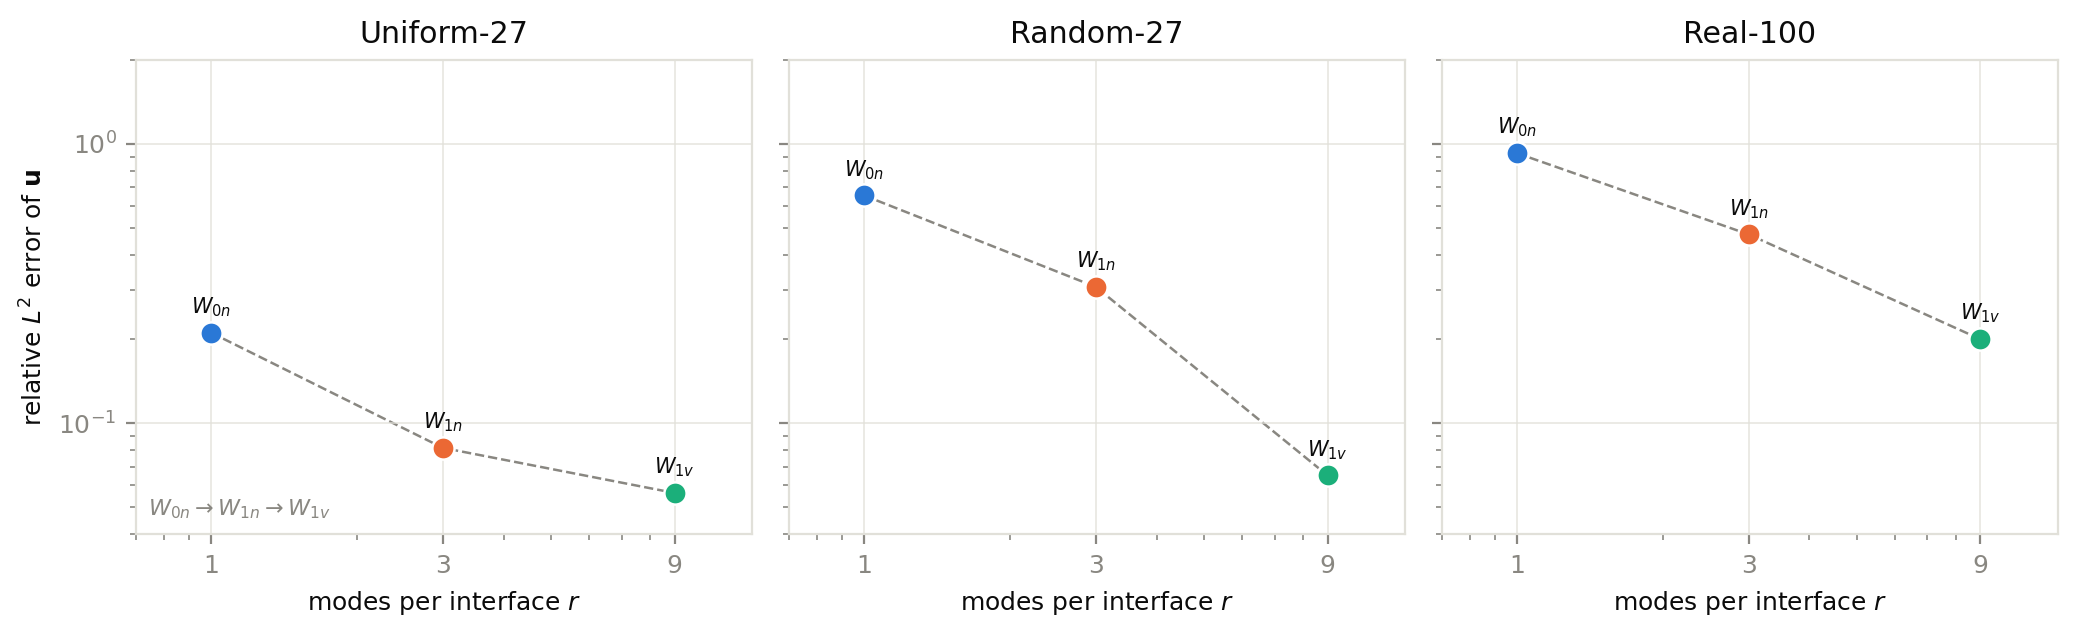
\includegraphics[width=0.97\textwidth]{figures/fig2_modal_budget.png}
  \caption{Relative $L^2$ velocity error versus modes per interface
    ($r=1,3,9$) along the nested path
    $\Wspace_{0n}\to\Wspace_{1n}\to\Wspace_{1v}$, for the three
    geometries (log scale).  Only the path through $\Wspace_{1n}$ was
    computed; the equal-budget space $\Wspace_{0v}$ at $r=3$ is
    planned work.}
  \label{fig:budget}
\end{figure}

The diminishing-returns shape ($1\to3$ much larger than $3\to9$) is
consistent across all three geometries, while the \emph{level} of the
remaining error at $r=9$ differs strongly: $5.6\%$, $6.5\%$, $20\%$.
This visual supports the claim that the modal budget requirement is
geometry-dependent, without over-interpreting the exact values
(no asymptotics in $r$ are claimed).

\subsection{Metric comparison across geometries}
\label{sec:metrics}

Fig.~\ref{fig:metrics} shows all four metrics as dot plots
(velocity $L^2$, broken $H^1$, pressure $L^2$, outlet-flux error) with
logarithmic ordinate; the wide dynamic range ($0.3\%$--$112\%$) is the
reason for the log scale.  The figure reproduces the Table~3 numbers in
a form where the cross-geometry pattern is visible at a glance: the
Classic-to-Affine spread widens from the regular to the irregular and
realistic cases in every metric except the pressure error, which stays
within one decade across all geometries and methods.

\begin{figure}[t]
  \centering
  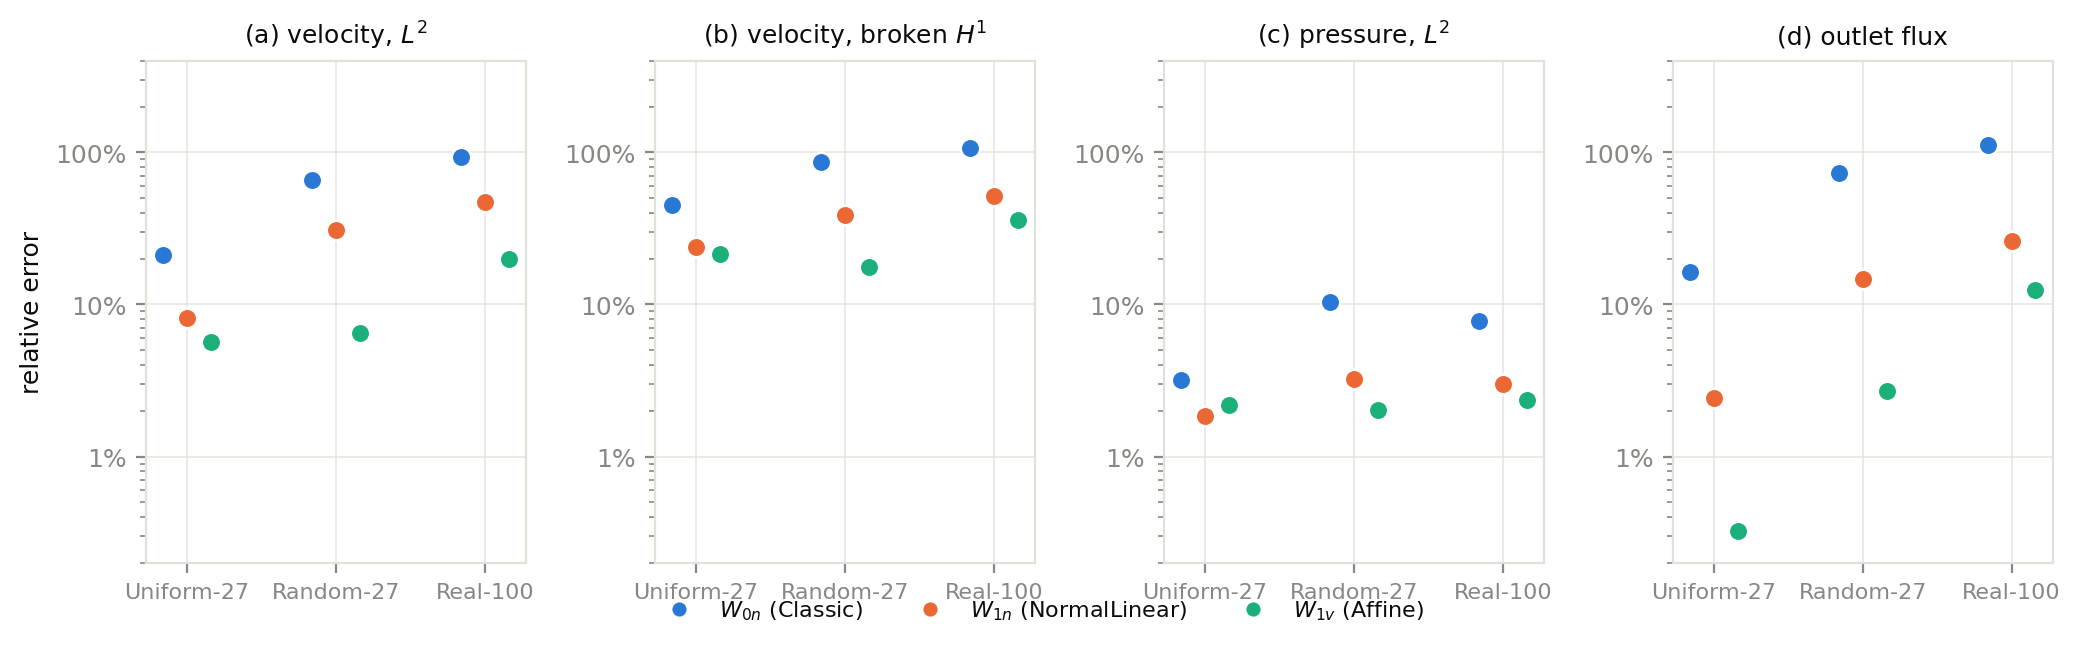
\includegraphics[width=0.97\textwidth]{figures/fig3_metrics.png}
  \caption{Four error metrics (relative, log scale) across the three
    geometries, three computed spaces: (a)~velocity $L^2$,
    (b)~velocity broken $H^1$, (c)~pressure $L^2$, (d)~outlet-flux
    error.}
  \label{fig:metrics}
\end{figure}

\subsection{Equal-budget comparison $\Wspace_{0v}$ vs.\ $\Wspace_{1n}$:
  planned}
\label{sec:equalbudget}

The central controlled contrast of the programme is the equal-budget
comparison
\begin{equation}
  G_{0v} = \frac{e_{0n}-e_{0v}}{e_{0n}}, \qquad
  G_{1n} = \frac{e_{0n}-e_{1n}}{e_{0n}},
\end{equation}
i.e.\ the FEM-relative $L^2$ reduction obtained by spending three DOFs
per interface on constant directional content ($\Wspace_{0v}$) versus
on first-order spatial content ($\Wspace_{1n}$).  This experiment was
\emph{not} run in the archived benchmarks (the constant-vector basis is
implemented in the four-space framework but no runs were executed).
It is the first item of \S10.3.  Until it is computed, the statement
that the normal-linear modes are the dominant mechanism rests on the
comparison $\Wspace_{0n}\to\Wspace_{1n}\to\Wspace_{1v}$ alone
(Fig.~\ref{fig:budget}), which cannot separate directional from spatial
information.

\subsection{Field visualization}
\label{sec:fields}

Fig.~\ref{fig:fields} shows, for Uniform-27 and Random-27, the mid-plane
slice $z=0.5$ of the FEM velocity magnitude together with the pointwise
velocity-error magnitude of the three reduced spaces.  Within each row
the three error panels share one color scale, so the reduced spaces are
directly comparable panel to panel; the reference panel has its own
scale.  Axes are the physical coordinates of the unit cube.  Solid
outlines mark the sections of the solid spheres, and grey lines the
intersections of the partition interfaces with the slice plane.  Along
the sequence $\Wspace_{0n}\to\Wspace_{1n}\to\Wspace_{1v}$ the error
becomes both weaker and more spatially localized.  On Uniform-27 the
normal-linear space $\Wspace_{1n}$ already recovers most of the
structure, while on Random-27 the residual $\Wspace_{1n}$ error is still
spread over extended regions and only the affine space $\Wspace_{1v}$
approaches the FEM field, consistent with the global metrics
(Table~\ref{tab:master}).

\begin{figure}[t]
  \centering
  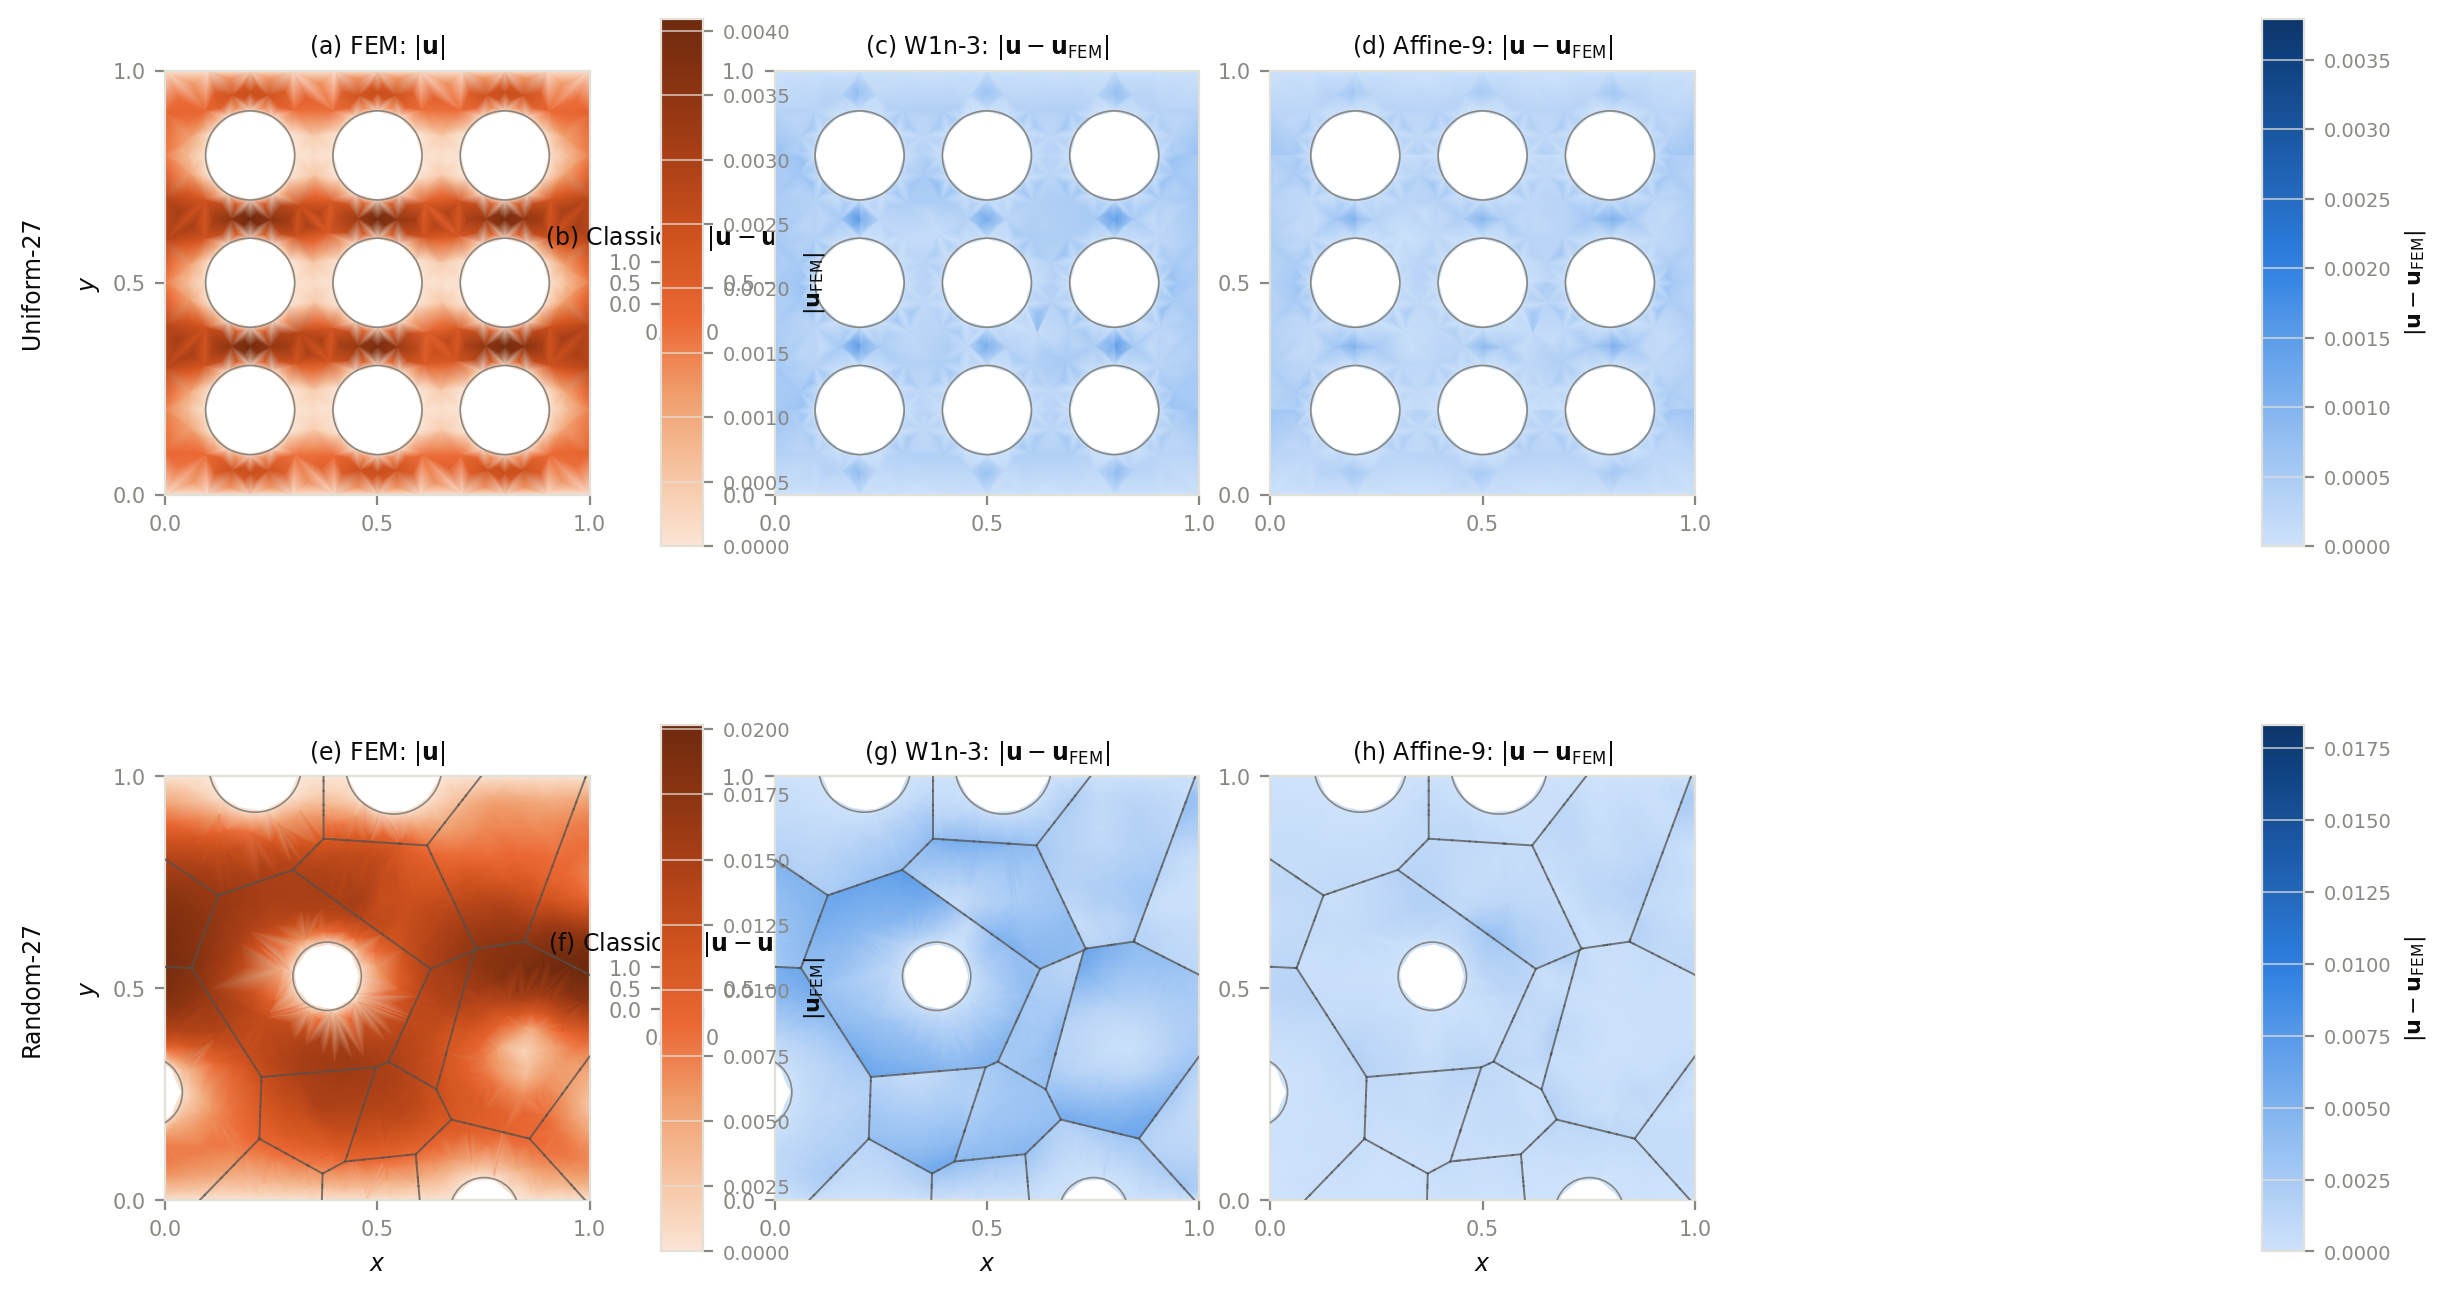
\includegraphics[width=0.97\textwidth]{figures/fig6_fields.png}
  \caption{Slice plane $z=0.5$ of the velocity field and the FEM-relative
    velocity error on Uniform-27 (top row) and Random-27 (bottom row).
    Panels (a,e) show the FEM velocity magnitude
    $|\mathbf{u}_{\rm FEM}|$; panels (b,f), (c,g) and (d,h) show
    $|\mathbf{u}-\mathbf{u}_{\rm FEM}|$ for $\Wspace_{0n}$,
    $\Wspace_{1n}$ and $\Wspace_{1v}$.  Coordinates are physical (unit
    cube).  Within each row the three error panels use a common color
    scale to enable direct visual comparison; the reference panel has
    its own scale.  Solid outlines are the sections of the solid spheres
    and grey lines the partition-interface intersections with the slice
    plane.}
  \label{fig:fields}
\end{figure}

The slice fields are available for the two controlled geometries;
per-interface normal-flux fields and Heterogeneous-100 field outputs
remain planned work (see \S\ref{sec:limitations}).

% ======================================================================
\section{Realistic porous structure (Real-100)}
\label{sec:realistic}
% ======================================================================

\subsection{Accuracy}
\label{sec:realacc}

The Real-100 geometry is the largest and most realistic of the three
(32\,611 cells, 166\,841 mixed DOFs, porosity $0.856$).  Its accuracy
rows in Table~\ref{tab:master} repeat the qualitative pattern of the
controlled geometries, at a higher level: Classic $\Wspace_{0n}$
misses $92.5\%$ of the velocity $L^2$ norm and even overshoots in the
broken $H^1$ seminorm ($e_u^{H^1_{\mathrm{br}}} = 1.063$); NormalLinear
reduces the $L^2$ error to $47.4\%$ and the flux error to $25.9\%$;
Affine reaches $e_u^{L^2}=20.0\%$, $e_Q=12.4\%$.  The pressure error is
the least sensitive metric here as well ($7.8\%\to3.0\%\to2.4\%$).
These are the least accurate of the three geometries for every space,
which is consistent with the larger fluid volume and the more
convoluted interface network, but no single descriptor is claimed to
explain the ordering.

\subsection{Cost and memory}
\label{sec:realcost}

Table~\ref{tab:cost} reports the cost structure of all runs.  For
Uniform-27 and Random-27 the reduced methods achieve a genuine
first-solve speedup over the monolithic FEM ($10.5\times$ and $13.3\times$
for Classic; $8.2\times$ and $9.1\times$ for Affine), because the
offline library is cheap relative to the FEM solve on those meshes.
For Real-100 the situation is reversed: the monolithic solve takes
$14.5\,$s while the reduced offline phase takes $28$--$33\,$s, so a
single reduced solve is \emph{slower} in wall time than the FEM solve;
only the online phase is fast ($0.06$--$1.4\,$s, i.e.\ $255\times$,
$72\times$, $10\times$ faster than the FEM solve).  The table therefore
states absolute times for both phases and both references, and the
speedup discussion is confined to the stated scopes.

Memory: peak footprints on Real-100 are $45$\,MiB (Classic),
$79$\,MiB (NormalLinear), $246$\,MiB (Affine) versus $300$\,MiB for the
monolithic solve; all fits comfortably in memory, and the growth with
the mode count is consistent with the $9m$ coupling block of the
Affine Schur matrix.

\begin{table}[t]
  \centering
  \small
  \caption{Computational cost (seconds).  $T_{\mathrm{offline}}$: local
    factorisations + primitive responses; $T_{\mathrm{online}}$:
    reduced assembly + Schur solve + reconstruction;
    $T_{\mathrm{first}} = T_{\mathrm{offline}}+T_{\mathrm{online}}$.
    FEM column = monolithic assembly+solve.  $N_{\mathrm{prim}}$ =
    primitive RHS columns.  For Real-100, $T_{\mathrm{first}}$ is the
    archived total; FEM there is the monolithic solve only.}
  \label{tab:cost}
  \begin{tabular}{llcccccc}
    \toprule
    Geometry & Method & unknowns & $N_{\mathrm{prim}}$ &
    $T_{\mathrm{offline}}$ & $T_{\mathrm{online}}$ &
    $T_{\mathrm{first}}$ & speedup vs FEM \\
    \midrule
    Uniform-27 & $W_{0n}$ & 144 & 320 & 7.35 & 0.0071 & 7.36 & $10.50\times$ \\
    Uniform-27 & $W_{1n}$ & 432 & 896 & 7.38 & 0.0222 & 7.40 & $10.44\times$ \\
    Uniform-27 & $W_{1v}$ & 1296 & 2624 & 9.18 & 0.208 & 9.39 & $8.23\times$ \\
    Uniform-27 & FEM & 63\,955 & -- & -- & 77.25 & 77.25 & $1\times$ \\
    \addlinespace[2pt]
    Random-27 & $W_{0n}$ & 114 & 246 & 8.90 & 0.0141 & 8.91 & $13.29\times$ \\
    Random-27 & $W_{1n}$ & 342 & 702 & 9.20 & 0.0287 & 9.22 & $12.84\times$ \\
    Random-27 & $W_{1v}$ & 1026 & 2070 & 12.82 & 0.191 & 13.01 & $9.10\times$ \\
    Random-27 & FEM & 75\,954 & -- & -- & 118.42 & 118.42 & $1\times$ \\
    Random-27 & Exact-FE-Schur & 21\,970 & -- & -- & 465.90 & 465.90 & $0.25\times$ \\
    \addlinespace[2pt]
    Real-100 & $W_{0n}$ & 144 & -- & 27.9 & 0.057 & 27.98 & $255\times$ (online only) \\
    Real-100 & $W_{1n}$ & 432 & -- & 28.0 & 0.203 & 28.17 & $72\times$ (online only) \\
    Real-100 & $W_{1v}$ & 1296 & -- & 32.7 & 1.400 & 34.13 & $10\times$ (online only) \\
    Real-100 & FEM & 166\,841 & -- & -- & 14.53 & 14.53 & $1\times$ \\
    \bottomrule
  \end{tabular}
  \medskip
  \raggedright\footnotesize
  Peak memory (Real-100 only): $W_{0n}$ 45.0, $W_{1n}$ 78.8,
  $W_{1v}$ 246.4, FEM 299.8\,MiB.  ``Online only'' speedups are
  $T_{\mathrm{online}}(\mathrm{FEM})/T_{\mathrm{online}}(X)$; the
  absolute times show that a single Real-100 reduced solve is slower
  than the FEM solve in wall time.
\end{table}

\subsection{Accuracy--cost tradeoff}
\label{sec:pareto}

Fig.~\ref{fig:pareto} plots, per geometry, the relative $L^2$ velocity
error against the online solve time on log--log axes, together with the
monolithic FEM reference point.  It answers the question ``what accuracy
does the added modal information buy'' in cost terms.  For all three
geometries the reduced points lie on a clear accuracy--cost frontier
above and to the left of the FEM point; the frontier is strongly
geometry-dependent (the Real-100 points at $r\ge3$ remain above the
Uniform-27 $r=1$ error).  The figure does \emph{not} include the
offline cost, which is the dominant part of $T_{\mathrm{first}}$ on
Real-100; it is shown because the online phase is the asymptotically
recurring cost in a many-query scenario, and the caption says so.

\begin{figure}[t]
  \centering
  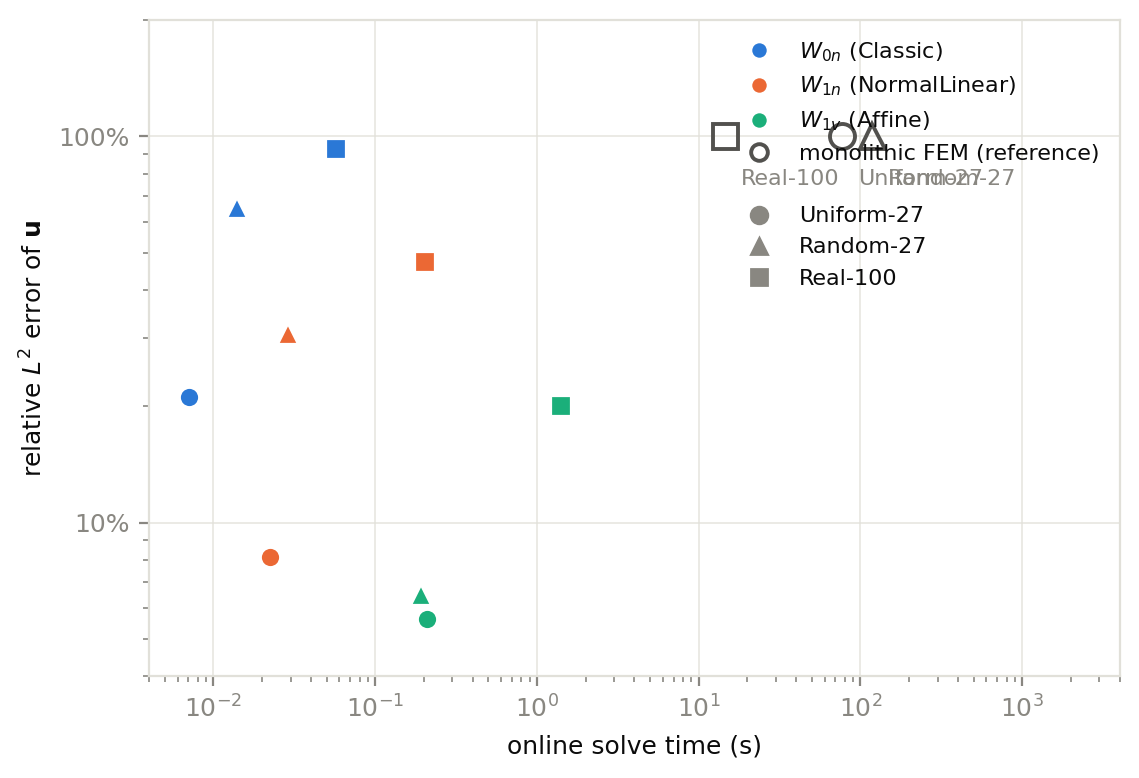
\includegraphics[width=0.62\textwidth]{figures/fig5_pareto.png}
  \caption{Relative $L^2$ velocity error versus online solve time
    (log--log).  Marker shape = geometry; colour = space (blue
    $\Wspace_{0n}$, orange $\Wspace_{1n}$, aqua $\Wspace_{1v}$);
    hollow markers = monolithic FEM reference.  Online time excludes
    the offline library phase (see Table~\ref{tab:cost}).}
  \label{fig:pareto}
\end{figure}

% ======================================================================
\section{Cross-geometry modal analysis}
\label{sec:cross}
% ======================================================================

\subsection{Observed FEM-relative error-reduction shares}
\label{sec:shares}

Along the computed path $\Wspace_{0n}\to\Wspace_{1n}\to\Wspace_{1v}$ the
observed FEM-relative $L^2$ velocity-error reduction decomposes into the
normal-spatial step ($\Wspace_{0n}\to\Wspace_{1n}$) and the additional
vectorial step ($\Wspace_{1n}\to\Wspace_{1v}$):
\begin{equation}
  R_N = \frac{e_{0n}-e_{1n}}{e_{0n}-e_{1v}}, \qquad
  R_{V|N} = \frac{e_{1n}-e_{1v}}{e_{0n}-e_{1v}}, \qquad
  R_N + R_{V|N} = 1.
  \label{eq:shares}
\end{equation}
Fig.~\ref{fig:shares} and Table~\ref{tab:cross} report these shares.

\begin{figure}[t]
  \centering
  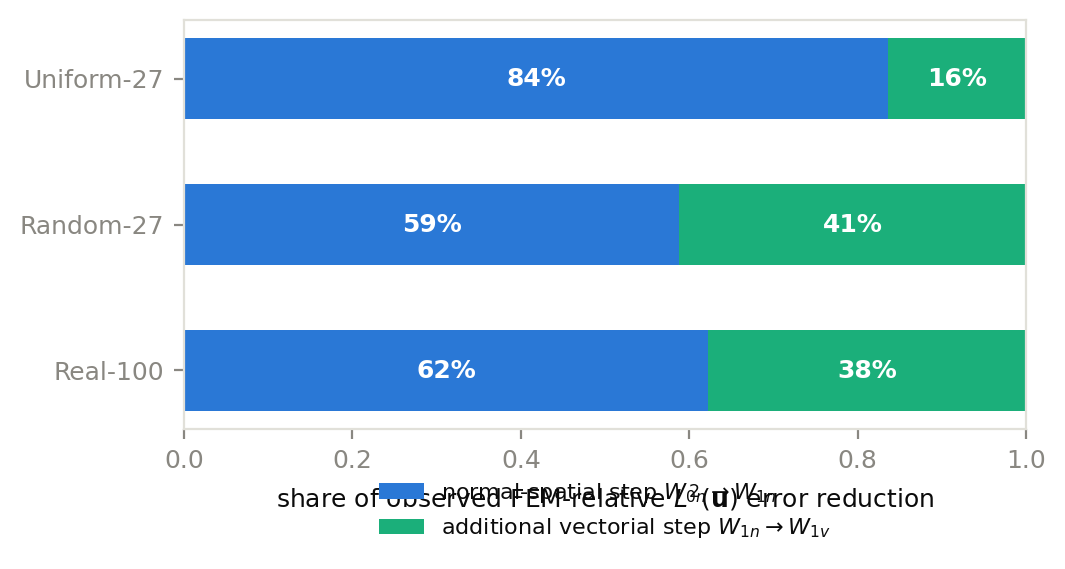
\includegraphics[width=0.55\textwidth]{figures/fig4_shares.png}
  \caption{Fractions of the \emph{observed} FEM-relative $L^2$ velocity
    error reduction along the prescribed path
    $\Wspace_{0n}\to\Wspace_{1n}\to\Wspace_{1v}$ (100\% stacked).
    These fractions are descriptive; they are not unique causal modal
    contributions, because the four middle spaces are generally
    non-nested and the path choice fixes the attribution.}
  \label{fig:shares}
\end{figure}

\begin{table}[t]
  \centering
  \small
  \caption{Cross-geometry modal summary: absolute errors and the
    observed FEM-relative reduction shares of \eqref{eq:shares}.}
  \label{tab:cross}
  \begin{tabular}{lcccccc}
    \toprule
    Geometry & $e_{0n}^{L^2}$ & $e_{1n}^{L^2}$ & $e_{1v}^{L^2}$ &
    $R_N$ & $R_{V|N}$ & reduction $\frac{e_{0n}-e_{1v}}{e_{0n}}$ \\
    \midrule
    Uniform-27 & 0.2108 & 0.0816 & 0.0563 & 83.6\% & 16.4\% & 73.3\% \\
    Random-27  & 0.6532 & 0.3075 & 0.0651 & 58.8\% & 41.2\% & 90.0\% \\
    Real-100   & 0.9254 & 0.4738 & 0.1998 & 62.2\% & 37.8\% & 78.4\% \\
    \bottomrule
  \end{tabular}
\end{table}

Two statements can be made from these numbers, both confined to the
tested configurations and to the chosen path:

\begin{enumerate}[label=\textbf{(D\arabic*)}.,leftmargin=*,nosep]
\item On all three geometries the normal-spatial step
  $\Wspace_{0n}\to\Wspace_{1n}$ accounts for the majority of the
  observed reduction ($59$--$84\%$).
\item The share of the vectorial step $\Wspace_{1n}\to\Wspace_{1v}$
  is markedly larger on the irregular/realistic geometries
  ($41\%$ and $38\%$) than on the regular lattice ($16\%$): the
  relative value of the additional directional content increases with
  geometric irregularity as measured by the variability descriptors of
  Table~\ref{tab:geometry} (Random-27 has the largest $\cov{A_\gamma}$
  and $\cov{a_\gamma/b_\gamma}$).  This is an observed association, not
  a proven causal relation.
\end{enumerate}

\subsection{Schur-energy pathwise decomposition: planned}
\label{sec:schurdecomp}

The theory sections give an \emph{exact} decomposition of the squared
Schur-energy error into pathwise marginal gains (see \S7.3).  Unlike
the FEM-relative shares of Fig.~\ref{fig:shares}, those quantities
($\Delta_N$, $\Delta_{T|N}$ etc.\ in the $\Shatuu$-seminorm) are
theorem-level and require the full C-DD trace solution
$\xiX{\mathrm{CDD}}$.  They were not computed in the archived runs and
are therefore not reported numerically; Fig.~\ref{fig:shares} and the
planned Schur-energy figure must not be conflated.  The former is an
observed descriptive attribution, the latter would be a strict theorem
quantity; only the former is available at this stage.

\subsection{Geometry dependence and limitations}
\label{sec:limitations}

\textbf{What the current data supports.}  (i)~constant-normal coupling
$\Wspace_{0n}$ is insufficient to represent the finite-area pore
interfaces accurately on any of the three geometries; (ii)~the
first-order normal modes $\Wspace_{1n}$ provide a major correction on
all three; (iii)~the residual gap between $\Wspace_{1n}$ and
$\Wspace_{1v}$ is small on the regular geometry and substantial on the
irregular/realistic ones, so the effective low-dimensional modal
requirement of an interface \emph{depends on the geometry across the
tested configurations}; (iv)~no monotonic dependence of the error on a
single scalar geometry descriptor is claimed.

\textbf{What is planned and not yet computed.}  (a)~the equal-budget
space $\Wspace_{0v}$ (constant tangential modes) on all three
geometries, enabling the controlled contrast of \S8.4;
(b)~the full C-DD solve $\xiX{\mathrm{CDD}}$ on Uniform-27 and
Random-27 for the exact Schur-energy verification (\S7.3) and the
pathwise decomposition (\S10.2); (c)~a mesh-sensitivity study
(Uniform-27 at three mesh levels) to confirm that the separation
$\Wspace_{0n}\gg\Wspace_{1n}>\Wspace_{1v}$ is not an artifact of one
mesh; the theory gives fixed-mesh separation only, no
mesh-independent asymptotic statement; (d)~an ensemble of random
realisations of the Random-27 geometry to test the stability of the
$59/41$ split across seeds; (e)~slice-field outputs for Real-100 once
the \texttt{z\_slice} interface mismatch is fixed; (f)~a second real
geometry at a different sphere count.

\textbf{Scope notes.}  All timings are single-machine, single-threaded
measurements from the archived runs; they are indicative, not
benchmark-suite grade.  The reported errors are with respect to the
monolithic Taylor--Hood FEM on the same mesh; the relation between the
broken-pressure C-DD discretisation and the monolithic system is not
established in the theory sections, and therefore no claim about the
accuracy of the reduced methods \emph{relative to the exact Stokes
solution} is made.

% ======================================================================
\section*{Appendix A: archived output provenance}
\label{app:provenance}
% ======================================================================

All numbers in this section were produced by the archived benchmark
runs of 2026-08-10 and are stored in
\begin{itemize}[nosep,leftmargin=*]
\item \texttt{affine\_ddpnm\_3d/outputs/benchmark\_w1n/}:\\
  \texttt{affine\_ddpnm\_metrics.csv}, \texttt{affine\_ddpnm\_report.json},
  \texttt{affine\_benchmark\_fields.npz};
\item \texttt{affine\_ddpnm\_3d\_random\_porous/outputs/benchmark\_w1n/}:\\
  \texttt{random\_affine\_metrics.csv}, \texttt{random\_affine\_report.json},
  \texttt{random\_benchmark\_fields.npz};
\item \texttt{real\_porous\_benchmark\_3d/outputs/benchmark\_w1n/}:\\
  \texttt{benchmark\_metrics.csv}, \texttt{benchmark\_report.json};
\item the base-project verification run\\
  \texttt{ddpnm\_3d\_uniform\_spheres/outputs/verify\_run/} (Classic
  Schur eigenvalue footnote).
\end{itemize}
Geometry descriptors were recomputed by the enclosed script
(\texttt{scripts/geometry\_stats.py}) directly from the saved
partition meshes (Uniform-27, Random-27) and by rebuilding the grid
partition with the benchmark's own builder (Real-100); the resulting
\texttt{data/geometry\_stats.json} accompanies this section.  All
figures were regenerated from the CSVs/JSON above by
\texttt{scripts/make\_figures.py}; the field panels of
Fig.~\ref{fig:fields} additionally use the two field archives listed
above; no numbers were edited by hand beyond rounding to the
significant digits shown.

% ======================================================================
\section*{Appendix B: archived benchmark plot (Uniform-27)}
\label{app:archived}
% ======================================================================

The benchmark pipeline itself produced the four-method comparison plot
shown in Fig.~\ref{fig:archived} (errors, speedup and offline time for
the Uniform-27 geometry), which we reproduce here as the archival
artifact it is; its bar-chart form is kept exactly as generated, and
the colour of the NormalLinear series (\#7B1FA2) follows the original
run, not the palette of the new figures.

\begin{figure}[t]
  \centering
  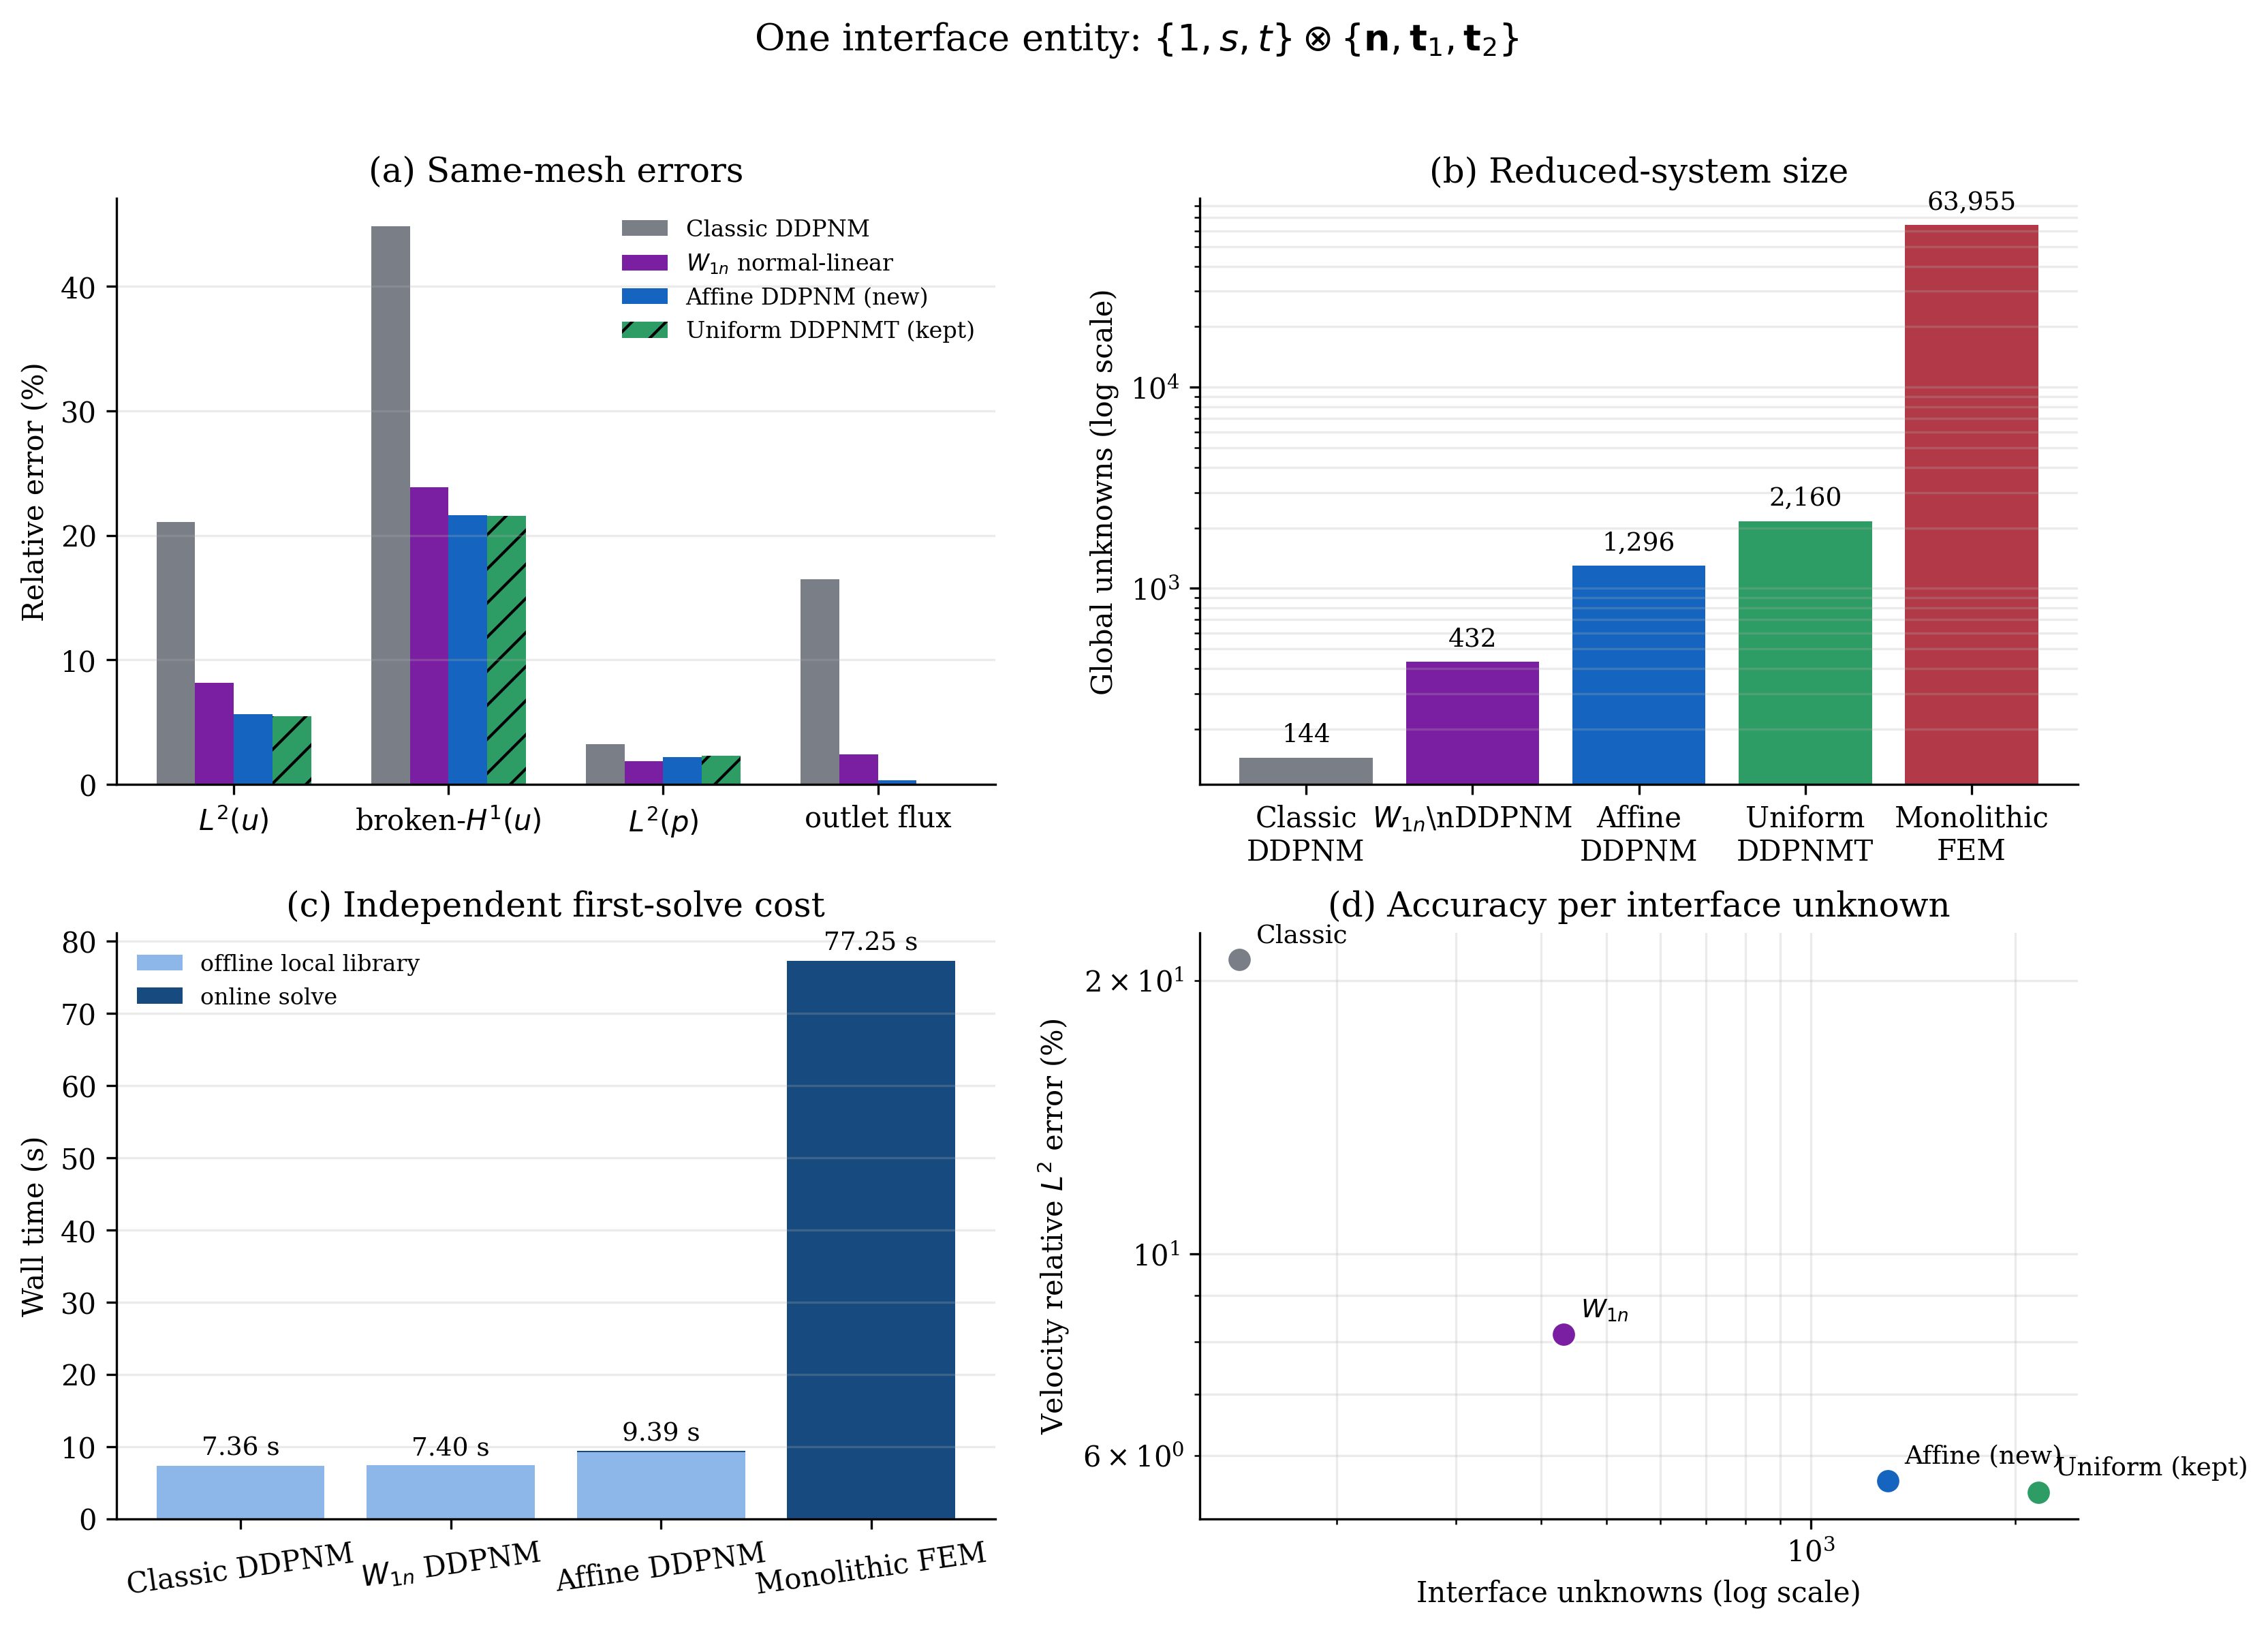
\includegraphics[width=0.95\textwidth]{figures/figA1_archived_uniform_comparison.png}
  \caption{Archived comparison plot generated by the Uniform-27
    benchmark run itself (Classic/W1n/Affine vs.\ FEM): relative errors
    (velocity $L^2$, broken $H^1$, pressure $L^2$, flux), speedup and
    offline time.  Reproduced unchanged.}
  \label{fig:archived}
\end{figure}

\end{document}
